\documentclass{article}

\usepackage{titlesec}
\usepackage{longtable}
\usepackage{array} % for defining a new column type
\usepackage{varwidth} %for the varwidth minipage environment
\usepackage{color, colortbl}
\usepackage{caption}
\usepackage{subfigure}
\usepackage{filecontents}
\usepackage[section]{placeins}
\usepackage{float}
\usepackage{lscape}

\definecolor{Gray}{gray}{0.9}

\usepackage{pgf-umlsd}
\usepackage{pgf-umlcd}
\newcommand{\sectionbreak}{\clearpage}

\begin{document}

\newcolumntype{M}{>{\begin{varwidth}{4cm}}l<{\end{varwidth}}} %M is for Maximal column

\begin{titlepage}
	\Huge{Bitcode Assignment 2}
\end{titlepage}


\section{Design Patterns}
Using design patterns in software project is a good practice. It helps to make your software understandable, sustainable and expendable. We have chosen two design patterns and implemented them in our existing code, the observer pattern and the factory pattern.

\subsection{The Observer Design Pattern}
The observer pattern is implemented between the MouseActionHandler class (subject) and the DragAnimation class (observer). The MouseActionHandler listens for mouse input in a given window. A object of the DragAnimation class is created when a mouse drag is registered and updated when the position of the mouse pointer changes. 
\paragraph{} We have chosen this pattern on this location because it enables us to create more observers for the MouseActionHandler in the future. Therefore it will save time to implement new features that need the MouseActionHandler class.
 

\subsubsection{Observer Class Diagram}
\begin{figure}[H]
	\centering
	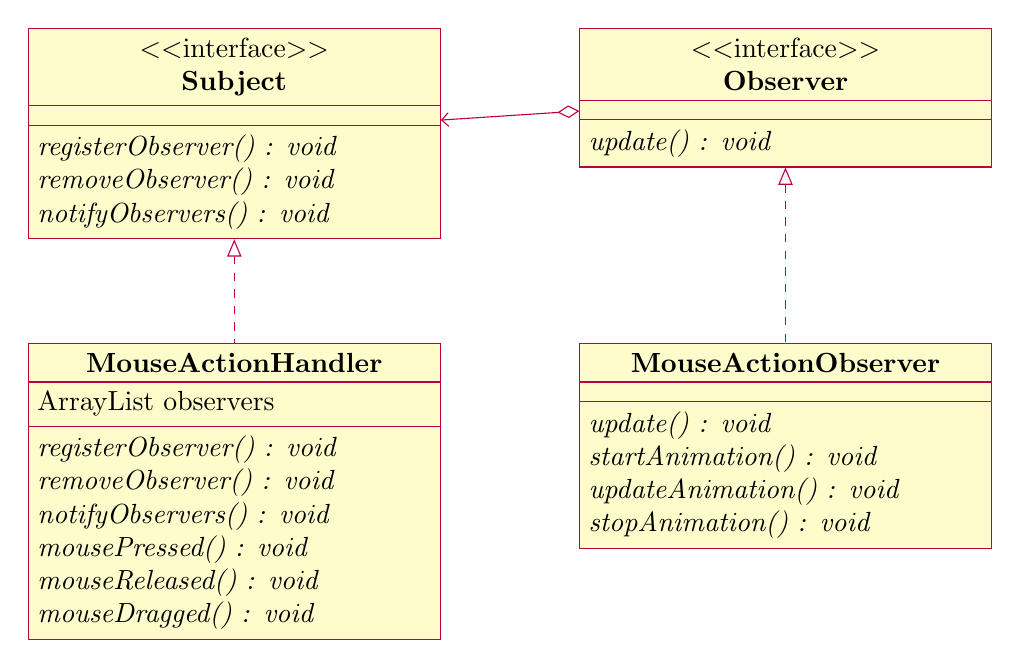
\begin{tikzpicture}
		\begin{interface}{Subject}{-3,0}
			\operation[0]{registerObserver() : void}
			\operation[0]{removeObserver() : void}
			\operation[0]{notifyObservers() : void}
		\end{interface}
		\begin{class}{MouseActionHandler}{-3,-4}
			\implement{Subject}
			\attribute{ArrayList observers}
			\operation[0]{registerObserver() : void}
			\operation[0]{removeObserver() : void}
			\operation[0]{notifyObservers() : void}
			\operation[0]{mousePressed() : void}
			\operation[0]{mouseReleased() : void}
			\operation[0]{mouseDragged() : void}
		\end{class}
		
		\begin{interface}{Observer}{4,0} 
			\operation[0]{update() : void}
		\end{interface}
		\begin{class}{MouseActionObserver}{4,-4}
			\implement{Observer}
			\operation[0]{update() : void}
			\operation[0]{startAnimation() : void}
			\operation[0]{updateAnimation() : void}
			\operation[0]{stopAnimation() : void}
		\end{class}
		
		\aggregation{Observer}{}{}{Subject}
		
	\end{tikzpicture}
\end{figure}

\newpage
\subsubsection{Observer Sequence Diagram}
\begin{figure}[H]
	\centering
	\begin{sequencediagram}
		\newinst[1]{C}{:DragAnimation}{}
		\newthread{A}{:MouseActionObserver}{}
		\newthread{B}{:MouseEventHandler}{}
		\begin{call}{A}{registerObserver()}{B}{}
		\end{call}
		\begin{sdblock}{Event}{mouse dragged}
			\begin{call}{B}{update()}{A}{}
				\begin{call}{A}{getMouseAction()}{B}{}
				\end{call}
				\begin{call}{A}{start()}{C}{}
				\end{call}
			\end{call}
		\end{sdblock}
	\end{sequencediagram}
\end{figure}

\subsection{The Factory Design Pattern}
The factory design patterns are implemented for the BoardFactory and the ItemFactory. On launch the board is created via the StandardBoardFactory which will construct a board using the StandardItemFactory.
\paragraph{} The reason that we have implemented a factory pattern for the Board class is that we can use this pattern in the future for creating different types of board. For instance creating boards with different sizes based on difficulty. 
\paragraph{} We have implemented the factory pattern for the Item class because that allows us to create different types of items in the board, such as special items that will remove all items from the board.

\subsubsection{Factory Class Diagram}
\begin{figure}[H]
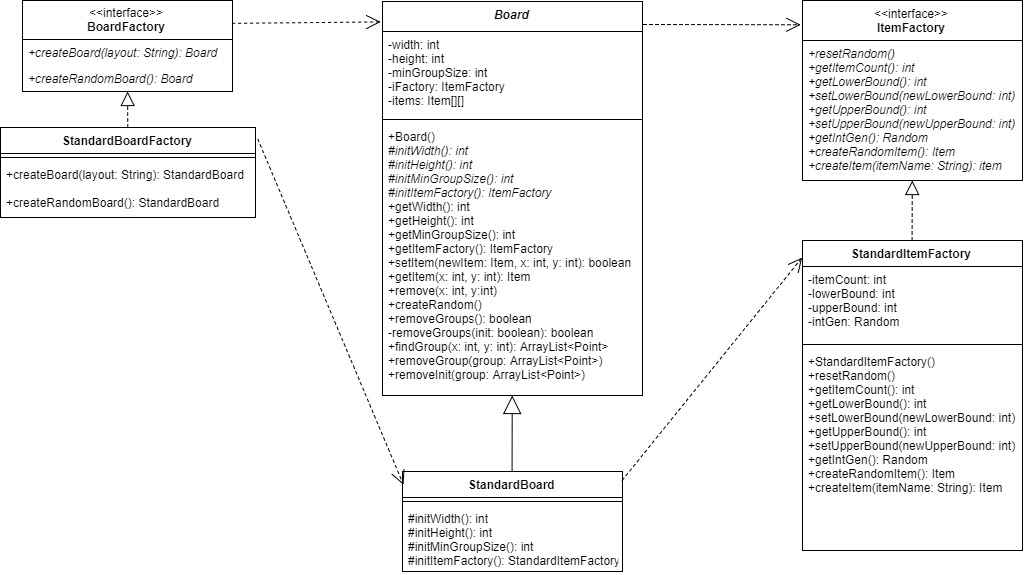
\includegraphics[scale=0.43]{Images/FactoriesClassDiagram.jpg}
\end{figure}

\subsubsection{Factory Sequence Diagram} 
\begin{figure}[H]
	\centering
	\begin{sequencediagram}
		\newthread{A}{:Game}{}
		\newinst[1]{B}{:StandardBoardFactory}{}
		\newinst[1]{C}{:StandardItemFactory}{}
		\begin{call}{A}{createBoard()}{B}{}
			\begin{call}{B}{Loop}{B}{}
				\begin{call}{B}{createItem()}{C}{}
				\end{call}
			\end{call}
		\end{call}
	\end{sequencediagram}
\end{figure}

\newpage
\section{Your wish is my command}
Our client wanted to have two new features implemented, which consist of a high score page and maximum amount of moves per level. For each each feature we have created new requirements and a software design.

\subsection{High Score Page}
tbd

\subsubsection{Requirements}
tbd

\subsubsection{Software Design}
tbd {use UML}

\subsection{Maximum Moves per Level}
Adding a constraint on the amount of moves in each level makes the game more immersive. The player needs to clear all items with a square background around them within a given number of moves. If the player manages to clear all these items within the maximum amount of moves the player will receive bonus points. When the player passes the amount of moves the player is able to continue the game to gain a higher score. 

\subsubsection{Requirements}
The requirement that can be subtracted are sorted using the MoSCoW model.

\paragraph{Must Haves}
\begin{itemize}
	\item There must be a maximum amount of moves per level.
	\item The player must receives bonus points when the player manages to remove all elements with a square background within the maximum amount of moves.
	\item The player must be able to continue the game after the amount of moves have passed. 
\end{itemize}
\paragraph{Should Haves}
\begin{itemize}
	\item The amount of moves should be configurable from the configuration file.
	\item The player should be able to see the amount of moves left.
\end{itemize}


\subsubsection{Software Design}
tbd {use UML} 


\section{Turn-based Multiplayer}
In exercise three we have been asked to implement a feature that we wanted to implement. We have chosen to implement turn-based Multiplayer. For this feature we also created new requirements and a software design.

\subsection{Requirements}
tbd

\subsection{Software Design}
tbd {use UML}



\end{document}






